\section{Data preprocessing}
Here we discuss how to process the traffic datasets. The overall process is illustrated in \figref{fig:data-processing}.

\begin{figure}[h!]
  \centering
    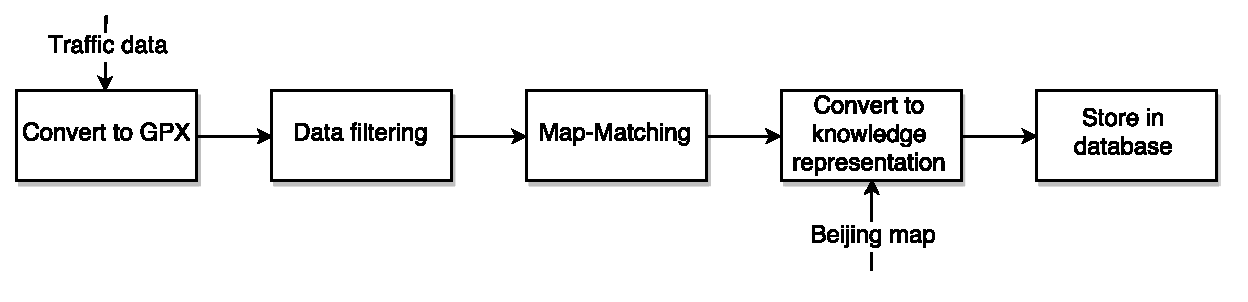
\includegraphics[width=1\textwidth]{figures/data_preprocessing.pdf}
    \caption{From raw gps data to database}
    \label{fig:data-processing}
\end{figure}

The GPS dataset is converted into the GPX format, which is then filtered to remove noise data. It is subsequently map-matched to the map of Beijing. The map-matched data and the Beijing map are then converted into their respective knowledge representations of the system, as described in \secref{sec:knowledge-representation}. Finally, the knowledge representation is stored in tables in the database.
By doing so, we have a knowledge base of the road network of Beijing and traffic data about vehicle movements, which we can learn traffic patterns from and find shortest paths for routes.

\subsection{Map generation}\label{sec:mapgeneration}
To model the road network of Beijing we need to have the specific information about all the roads in the road network. This information is available several places, but most of these services are not free. We have chosen to work with OpenStreetMap which is an open source map service, where users collaborate to keep the city maps updated. There are some problems in using this kind of service, such as the possibility of wrong data, limited data, since the map is updated by users, so it is possible for a user to make erroneous updates. Furthermore it is illegal for unauthorized persons to collect geographical data in China\cite{chinamapillegal}. But because this service was the only free service that we could find, we see no other option than having in mind that these problems can occur.

We have also found that the OpenStreetMap site cannot export large areas of a map, such as the whole city of Beijing. Therefore we have chosen to use one of its mirror sites, Geofabrik\cite{geofabrik}, which provides map extracts of the world, segmented into countries and these are updated daily. This makes it possible for us to extract the whole map for China.

\subsubsection{Format \& Pre-processing}
\label{chap:FormatPre-processing}
The maps from Geofabrik comes in a compressed format called pbf. To extract the relevant data from this format we are using a tool called Osmosis, to query the file using several filters to be able to extract only the relevant information.

We are using two types of filters with Osmosis, the first is used to set bounds on the area that we want to extract information from, these bounds are set as north, west, south and east in longitude and latitude. This filter is used since the map we are using is all of China and we are only interested in the road network of Beijing.

The second filter is used to extract only roads from the previous bounded area. With this filter we have the possibility to specify which roads we want to get in the output. Because all paths are marked in OpenStreetMap as ways, we want to filter these in order to remove side-walks, bicycle ways, and other ways that are not possible use by car or other motorized vehicles.

The extracted data from the Osmosis query is then exported to a file in XML format. There are two types left in the export, which are nodes and ways, as shown in the example \coderef{wayexample}. Nodes represent road intersections and are also used to indicate points along a road if the road is not straight. Both nodes and ways can include key-value pairs that contain information, i.e. if a way is one-way, if a traffic light is present at a given node. Ways also contain a nd tag, with id, for every node it consists of.

\begin{lstlisting}[style=Java, caption=An simplified example of a road and its related nodes in XML, label=wayexample]
<node id="388002830" lat="39.9931617" lon="116.4469860"/>
<node id="822458510" lat="39.9893342" lon="116.4477929"/>
<node id="822458512" lat="39.9901233" lon="116.4476014"/>
<node id="822458513" lat="39.9883905" lon="116.4481454"/>
<node id="822458514" lat="39.9877410" lon="116.4491191"/>
<node id="822458515" lat="39.9876340" lon="116.4493937"/>
<node id="2391519066" lat="39.9922187" lon="116.4471224"/>
<way id="230684654">
    <nd ref="388002830"/>
    <nd ref="2391519066"/>
    <nd ref="822458512"/>
    <nd ref="822458510"/>
    <nd ref="822458513"/>
    <nd ref="822458514"/>
    <nd ref="822458515"/>
    <tag k="highway" v="tertiary"/>
</way>
\end{lstlisting}

\subsubsection{Generation}
An XML parser is used to extract the information from the Osmosis export that is needed to model the road network. When a node or way tag is read an equivalent data structure is created and stored (see \coderef{lst:node} and \coderef{lst:way}).

\begin{lstlisting}[style=java, caption=Datastructure for a node, label=lst:node]
Node{
	long id;
	double longitude;
	double latitude;
	Way[] connectedWays;
}
\end{lstlisting}

\begin{lstlisting}[style=java, caption=Datastructure for a way, label=lst:way]
Way{
	long id;
	Node[] connectedNodes;
	int type;
}
\end{lstlisting}

A distinction between nodes have been made such that there are two kinds of nodes, one kind is points along a road and another are intersection nodes. Intersection nodes are either the nodes at the start or end of a road, or nodes that are intersections between ways. Using these nodes we create a class, Edge (see \coderef{lst:edge}, which is a edge between every pair of concequtive nodes on a way. But since the nodes there are points along a road does not add any information for a part of a way, we have also created the class, Segment (see \coderef{lst:segment}, which is an edge between every pair of intersection nodes on a way.

An example is show in \figref{fig:waywithnodes} which is an illustration of the way from \coderef{wayexample}. The orange line describes the way, the red and green points describe nodes, where the red points are intersection nodes and the green are points along a way. The black lines describe our edges and the blue lines describe our segments.

\begin{figure}[h!]
  \centering
    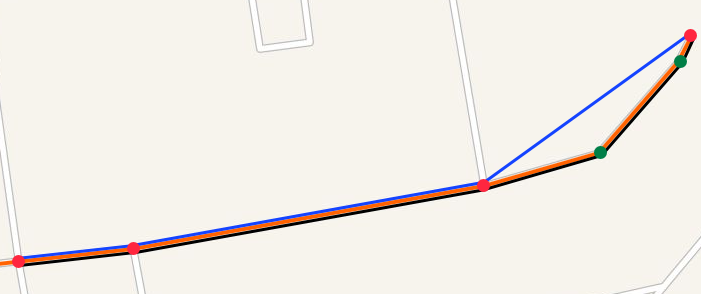
\includegraphics[width=0.8\textwidth]{figures/way-w-nodes2.png}
    \caption{A way with nodes}
    \label{fig:waywithnodes}
\end{figure}


\begin{lstlisting}[style=java, caption=Datastructure for an edge, label=lst:edge]
Edge{
	long id;
	double length;
	long origin;
	long destination;
	long segment;
}
\end{lstlisting}

\begin{lstlisting}[style=java, caption=Datastructure for a segment, label=lst:segment]
Segment{
	long id;
	double length;
	long way;
	long origin;
	long destination;
}
\end{lstlisting}

The relation between edges and segments is that each edge of a segment contains a reference to the segment that it is a part of, the same is true from the relation between ways and segments.

\subsection{Data filtering}\label{sec:datafiltering}
% WHAT IS IT?
% WHY DO WE DO IT?
% HOW DO WE DO IT?
We perform a simple spatial and temporal filtering on the GPS data to remove GPS samples outside the physical city limits. Filtering the data before further processing is key, since not all of the data is accurate or even useful for reasoning about the traffic. Even though the data that is filtered is reliable enough, we delimit our focus on congestion to the city center. Since most of the data is clustered in the city center anyway, we do not lose significant parts of the dataset by filtering these samples.

Furthermore, some GPS samples are of very bad quality. Some routes are (according to the GPS samples) at one moment driving through Beijing, and the next moment suddenly driving in Africa or Europe. This phenomenon could be caused by weak connection to the GPS satellites e.g. when driving through a tunnel. The inaccuracies these corrupt samples introduce, are taken care of as well by filtering samples outside of the city limits. Fortunately, we do not lose all of the samples associated with the rest of the route involved - just the corrupted sample.

\subsection{Map matching}\label{sec:mapmatching}
Generally, GPS coordinates measured are often imprecise due to external factors, and do therefore not reflect the precise location of, in this case, a vehicle. Consequently, the samples of the training set must be treated as approximations of GPS locations. This causes some problems in terms of how we should decide which road the vehicle was traveling on and what its speed was.

\begin{figure}
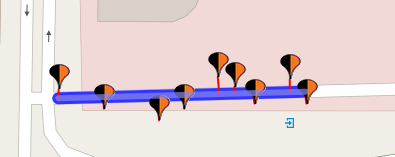
\includegraphics[scale=1]{figures/mapmatching.png}
\caption{GPS samples and the actual road driven on.}
\label{fig:mapmatching}
\end{figure}

The problem is illustrated in \figref{fig:mapmatching}. The orange-and-black colored GPS samples are imprecise in the sense that they are not mapped directly onto the blue road. The straightforward solution would just be to map the samples to the road closest to the collection of samples. However if the road network is dense, we can have multiple candidates for roads, since the distance from the samples to the two roads might be equal.

Consequently, we must perform the process of \emph{map-matching} the dataset of GPS samples to the most likely roads that vehicles was traveling on. Several algorithms and implementations exist that perform this task, including TrackMatching\cite{TrackMatching}, GraphHopper\cite{GraphHopper} and N-Gemma\cite{NGemma}. Limited informal evaluations of these implementations showed that TrackMatching provided a more precise map-matching than GraphHopper, both of which work with GPX-formatted GPS samples. Unfortunately, the documentation for N-Gemma was incomplete, and as such, we decided to not investigate further the use of N-Gemma, since TrackMatching was an adequate solution to the map-matching problem, despite it being a webservice.

Alternatively, we considered implementing a map-matching algorithm ourselves, however given that the focus of the project is on constructing an intelligent routing agent; not an efficient map-matching algorithm, we decided that our time would be better spent elsewhere, and opted for utilising an existing implementation for map-matching.

\subsubsection{TrackMatching input and output}
We chose to use the GPX format for input and GeoJSON as the output of the map-matcher. The output is represented as a tree structure in \figref{fig:geojson}. The \emph{links} element of each \emph{route} is an array of link objects.

\begin{figure}[H]
	\centering
	\begin{tikzpicture}
	\node {(root)}
	[
		level distance=1cm,
		level 1/.style={sibling distance=2cm},
		level 2/.style={sibling distance=1.5cm}
	]
	child { node {diary}
		child { node {entries}
			child { node {$\text{route}_\text{1}$}
				child { node {$\text{links}_\text{1}$}
					edge from parent [->] node [left] {}
				}
				edge from parent [->] node [left] {}
			}
			child { node {...}
				child { node {...}
					edge from parent [->] node {}
				}
				edge from parent [->] node {}
			}
			child { node {$\text{route}_\text{n}$}
				child { node {$\text{links}_\text{n}$}
					edge from parent [->] node [right] {}
				}
				edge from parent [->] node [right] {}
			}
			edge from parent [->] node {}
		}
		edge from parent [->] node [left] {}
	}
	child { node (a) {options}
		edge from parent [->] node {}
	}
	child { node [right=0.5cm of a] {performanceIndicators}
		edge from parent [->] node [right] {}
	}
	;
	\end{tikzpicture}
	\caption{Structure of GeoJSON output.}
	\label{fig:geojson}
\end{figure}

A simple example of a link object can be seen in \coderef{lst:geojson:link}. The \textbf{err} (error) attribute describes how accurately the waypoints were matched to a way; the lower the error, the more likely that the correct way was picked. The \textbf{src} (source) and \textbf{dst} (destination) attributes correspond to nodes in the map on the same way, which is identified through the \textbf{id} attribute (i.e., nodes \#src and \#dst are on way \#id). The source node in the next link is the destination node in the previous link, except for the first link. The coordinates in the \textbf{geometry} attribute contains the longitudes and latitudes projected to the EPSG:3857 coordinate reference system for each node that is passed through in the link. The \textbf{wpts} (waypoints) attribute contains the coordinates, id (within the link) and timestamp for each waypoint matched to the link. \todo{mangler noget her: hvorfor er det interessant? HVad bliver de forskellige dele brugt til?}

\begin{lstlisting}[style=java, caption=Content of a simple link object., label=lst:geojson:link]
{
  "err":398.43,
  "src":2639384604,
  "dst":2639384636,
  "id":258604821,
  "geometry":"{\"type\": \"LineString\", \"coordinates\": [[1.2997645E7, 4836996],[1.2997724E7, 4837050],[1.2997795E7, 4837084.5],[1.2997899E7, 4837123]]}",
  "wpts":[{
    "x":1.2997645E7,
    "y":4836996,
    "id":"0",
    "timestamp":"2008-02-02T15:10:20Z"
  },
  {
    "x":1.2998036E7,
    "y":4837174,
    "id":"1",
    "timestamp":"2008-02-02T15:10:25Z"
  }]
}
\end{lstlisting}
